% !TEX program = XeLaTeX
%%=======================================================================
%% HUAS-Beamer-Blue.tex —— 湖南文理学院 Beamer 模板「冷色调（蓝白）」中文演示
%%=======================================================================
%% 与 HUAS-Beamer.tex 内容相同，仅主题加载一行改为 [blue] 冷色调选项。
%% 蓝白配色定义见 huasbeamer.sty「色彩系统」区 \ifhuas@blue 分支。
%% 编译：xelatex HUAS-Beamer-Blue.tex（含参考文献需 xelatex → bibtex → xelatex ×2）
%%
%% ★ 如何改成你自己的 PPT ★（同 demo-cn.tex）
%%   1. 封面信息：\title / \subtitle / \author / \supervisor / \institute / \date
%%   2. 正文结构：\section / \subsection / \begin{frame}{标题}...\end{frame}
%%   3. 颜色/尺寸/图片/字体：见 huasbeamer.sty 的 ★注释★ 与 docs/模板使用与自定义说明.md
%%   4. 本页内容均为排版范例，可整段替换
%%=======================================================================
\documentclass[aspectratio=169]{beamer} % 16:9；4:3 改为去掉 aspectratio

% 图片路径（校徽、校标、建筑线稿已整理于 figures/）
\graphicspath{{figures/}}

% 加载 HUAS 主题（blue = 冷色调蓝白版；其余可选项：en / notoc / subsectiontoc / nonav）
\usepackage[blue]{huasbeamer}

% 常用宏包（按需增删）
\usepackage{listings}
\usepackage{multicol}
\usepackage{multirow}

\lstset{
  basicstyle=\ttfamily\scriptsize,
  keywordstyle=\bfseries\color{huasdeep},
  commentstyle=\itshape\color{huascoral},
  stringstyle=\color{huasorange},
  numbers=left,
  numberstyle=\tiny\color{gray},
  frame=single,
  rulecolor=\color{huasred!40},
  breaklines=true,
  aboveskip=0.2ex,
  belowskip=0.2ex,
}

%% ---------------- 封面信息（★内容填写★）----------------
\title[自读课文的教学]{浅谈自读课文的教学}       % [页脚短标题]{封面标题}
\subtitle{——以部编版八年级下册第二、四单元为例}  % 副标题（可删）
\author[张同学]{答辩人：张同学}                   % [页脚短作者]{封面作者}
\supervisor{指导教师：李老师\quad 教授}            % 导师行（可删整行）
\institute[湖南文理学院]{\small 湖南文理学院·文学院}
\date{\small 2025 年 6 月}

\begin{document}

%% ---------------- 封面 ----------------
\begin{frame}[plain,noframenumbering]
  \titlepage
\end{frame}

%% ---------------- 目录 ----------------
\begin{frame}{目录}
  \tocbackground % 目录页背景：校门线稿（定义于 huasbeamer.sty）
  \vskip-2em % ★位置★ 总目录整体上移
  {\setbeamerfont{section in toc}{size=\large}% ★字号★ 总目录条目加大
   \tableofcontents[hideallsubsections]}
\end{frame}

%% ==================== 一、研究背景与意义 ====================
\section{研究背景与意义}

\subsection{研究背景}

\begin{frame}{研究背景}
  \begin{block}{政策背景}
    \begin{itemize}
      \item 部编本语文教材构建了「教读—自读—课外阅读」三位一体阅读体系；
      \item 自读课文承担着从「教师引导」向「学生自主阅读」过渡的关键功能；
      \item 课程标准强调培养学生的独立阅读能力与阅读兴趣。
    \end{itemize}
  \end{block}
  \begin{alertblock}{现实困境}
    \begin{itemize}
      \item 自读课文教学「教读化」：逐段精讲、面面俱到；
      \item 学生主体地位缺失，阅读策略迁移不足。
    \end{itemize}
  \end{alertblock}
\end{frame}

\subsection{研究意义}

\begin{frame}{研究意义}
  \begin{columns}[T]
    \begin{column}{0.48\textwidth}
      \begin{exampleblock}{理论意义}
        \begin{itemize}
          \item 丰富自读课文教学的理论研究；
          \item 为「三位一体」阅读体系提供实践注脚。
        \end{itemize}
      \end{exampleblock}
    \end{column}
    \begin{column}{0.48\textwidth}
      \begin{exampleblock}{实践意义}
        \begin{itemize}
          \item 为一线教师提供可操作的教学策略；
          \item 促进学生阅读能力的自主建构。
        \end{itemize}
      \end{exampleblock}
    \end{column}
  \end{columns}
  \vskip1ex
  {\footnotesize\color{huasdeep}%
    引自《义务教育语文课程标准（2022 年版）》\cite{xkb2022}。}
\end{frame}

%% ==================== 二、研究内容与方法 ====================
\section{研究内容与方法}

\subsection{研究内容}

\begin{frame}{研究内容}
  \begin{itemize}[<+-| alert@+>]
    \item 梳理部编版八年级下册第二、四单元自读课文的编排特点；
    \item 调查当前自读课文教学的现状与问题；
    \item 提出自读课文教学的基本原则与实施策略；
    \item 结合具体课例进行教学设计与实践反思。
  \end{itemize}
  \vskip1.5ex
  \begin{block}{核心概念}
    自读课文：以学生自主阅读为主、教师点拨为辅，强调阅读方法迁移的课文类型
    \cite{wang2019}。
  \end{block}
\end{frame}

\subsection{研究方法}

\begin{frame}{研究方法}
  \begin{table}
    \centering\small
    \caption{研究方法一览}\label{tab:method}
    \begin{tabular}{lll}
      \huastableheader % 彩色表头行（huasbeamer 提供的 \huastableheader 宏）
      \huastableheaderfont 方法 & \huastableheaderfont 对象/样本 & \huastableheaderfont 目的 \\
      \midrule
      文献研究法 & 期刊论文 42 篇 & 梳理研究现状 \\
      问卷调查法 & 师生样本 320 份 & 把握教学现状 \\
      课堂观察法 & 课例 12 个 & 分析教学行为 \\
      案例分析法 & 教学设计 6 例 & 提炼实施策略 \\
      \bottomrule
    \end{tabular}
  \end{table}
\end{frame}

\subsection{单元选文概况}

\begin{frame}{单元选文概况}
  \begin{columns}[T]
    \begin{column}{0.55\textwidth}
      \begin{table}
        \centering\small
        \caption{第二、四单元选文分布}\label{tab:unit}
        \begin{tabular}{lccc}
          \huastableheader
          \huastableheaderfont 单元 & \huastableheaderfont 课文总数 &
          \huastableheaderfont 自读篇目 & \huastableheaderfont 占比 \\
          \midrule
          第二单元 & 5 & 2 & 40\% \\
          第四单元 & 5 & 2 & 40\% \\
          \midrule
          合计 & 10 & 4 & 40\% \\
          \bottomrule
        \end{tabular}
      \end{table}
    \end{column}
    \begin{column}{0.42\textwidth}
      \begin{center}
        
\includegraphics[width=0.42\textwidth]{huas-badge.png}
      \end{center}
      {\footnotesize\color{huasdeep}湖南文理学院}\\[0.5ex]
      {\scriptsize 自读篇目如《大自然的语言》《大雁归来》等，\\
        以说明性、议论性文本为主，突出方法迁移。}
    \end{column}
  \end{columns}
\end{frame}

\subsection{数据处理示例}

\begin{frame}[fragile]{数据处理示例}
  \vspace{-1.2ex}
  \begin{block}{问卷数据统计（节选）}
    以班级为单位统计阅读自我效能感得分均值（$n=320$）：
    \begin{equation}
      \bar{X} = \frac{1}{n}\sum_{i=1}^{n} x_i,
      \qquad
      S = \sqrt{\frac{1}{n-1}\sum_{i=1}^{n}(x_i-\bar{X})^2}
      \label{eq:mean}
    \end{equation}
    实验前后差异采用配对 $t$ 检验\cite{li2021}。
  \end{block}
  \vspace{-0.8ex}
  \begin{exampleblock}{分析脚本（节选）}
\begin{lstlisting}[language=Python]
import pandas as pd
data = pd.read_excel("reading_survey.xlsx")
mean, std = data["score"].mean(), data["score"].std()
print(f"mean = {mean:.2f}, std = {std:.2f}")
\end{lstlisting}
  \end{exampleblock}
\end{frame}

%% ==================== 三、教学策略与实践 ====================
\section{教学策略与实践}

\subsection{教学原则}

\begin{frame}{自读课文教学的基本原则}
  \begin{enumerate}
    \item \textbf{学生主体原则}——把课堂时间还给学生阅读；
    \item \textbf{方法迁移原则}——将教读课习得的策略迁移至自读课；
    \item \textbf{以评促读原则}——用阅读任务单、读书报告等评价驱动阅读；
    \item \textbf{整合拓展原则}——打通课内自读与课外整本书阅读。
  \end{enumerate}
  \vskip2ex
  \begin{block}{「旁批」的支架作用}
    自读课文的旁批为学生提供了思维支架，教学中应引导学生\emph{借助旁批
      学会提问}，逐步走向独立阅读。
  \end{block}
\end{frame}

\subsection{教学设计示例}

\begin{frame}{教学设计示例：《大雁归来》}
  \begin{columns}[T]
    \begin{column}{0.52\textwidth}
      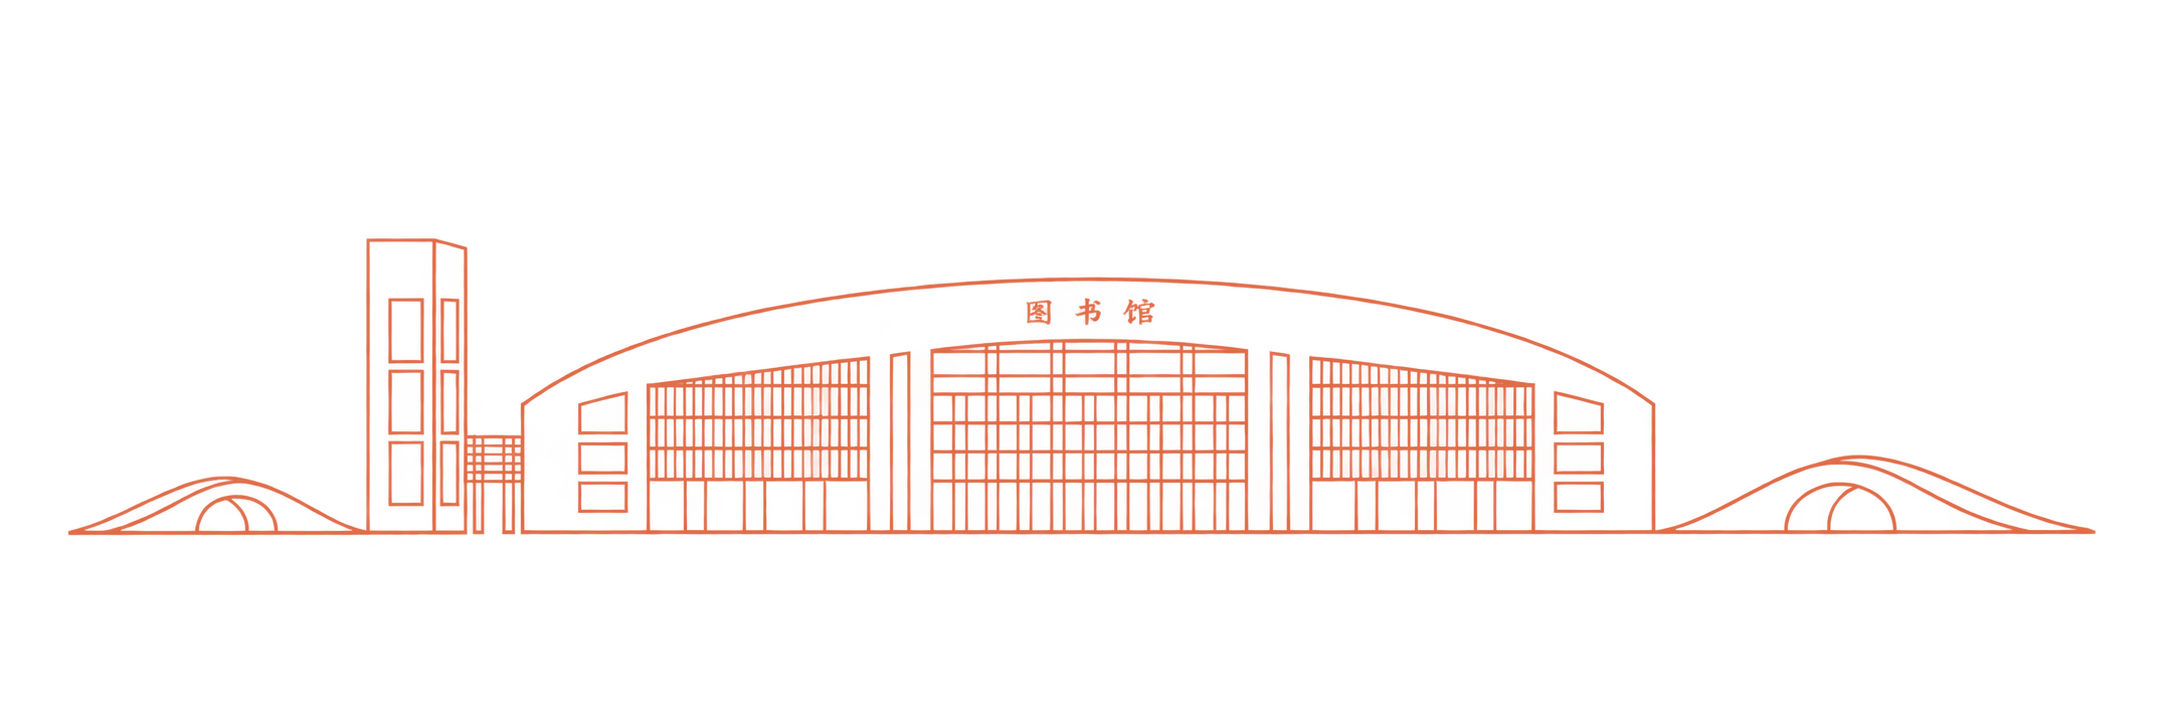
\includegraphics[width=\textwidth]{building-library.png}\\[0.5ex]
      {\scriptsize\color{huascoral}图：湖南文理学院图书馆（素材示意）}
    \end{column}
    \begin{column}{0.44\textwidth}
      \small
      \begin{description}
        \item[导入] 候鸟迁徙短视频引入；
        \item[自读] 借助旁批完成任务单；
        \item[交流] 小组汇报、质疑答辩；
        \item[迁移] 比较阅读《大自然的语言》；
        \item[作业] 撰写 300 字观察笔记。
      \end{description}
    \end{column}
  \end{columns}
\end{frame}

\subsection{实践效果}

\begin{frame}{实践效果}
  \begin{block}{课堂观察结论}
    \begin{itemize}
      \item 学生自主阅读时长由 8 分钟提升至 18 分钟；
      \item 课堂提问中「学生主动提问」占比由 21\% 提升至 57\%；
      \item 阅读策略迁移任务完成率提升 32\%。
    \end{itemize}
  \end{block}
  \begin{alertblock}{需要注意}
    自读不等于「放手」，教师的点拨与反馈仍是质量保障的关键环节。
  \end{alertblock}
\end{frame}

%% ==================== 四、总结与展望 ====================
\section{总结与展望}

\begin{frame}{结论与展望}
  \begin{block}{研究结论}
    \begin{itemize}
      \item 自读课文教学应回归学生自主阅读的本位；
      \item 任务单 + 旁批支架 + 比较阅读是行之有效的策略组合；
      \item 「教读—自读—课外阅读」的一体化设计值得深入探索。
    \end{itemize}
  \end{block}
  \begin{exampleblock}{后续工作}
    \begin{itemize}
      \item 扩大样本，开展准实验研究；
      \item 探索信息技术支持下的自读课堂评价。
    \end{itemize}
  \end{exampleblock}
\end{frame}

%% ---------------- 参考文献 ----------------
\begin{frame}[allowframebreaks]{参考文献}
  \footnotesize
  \bibliographystyle{plain}
  \bibliography{reference}
\end{frame}

%% ---------------- 致谢 / Q&A ----------------
\begin{frame}[plain,noframenumbering]
  \begin{tikzpicture}[remember picture,overlay]
    \shade[left color=huasdeep,right color=huasorange]
      (current page.south west) rectangle (current page.north east);
    \node[anchor=south,opacity=0.16] at ([yshift=0.35cm]current page.south) {%
      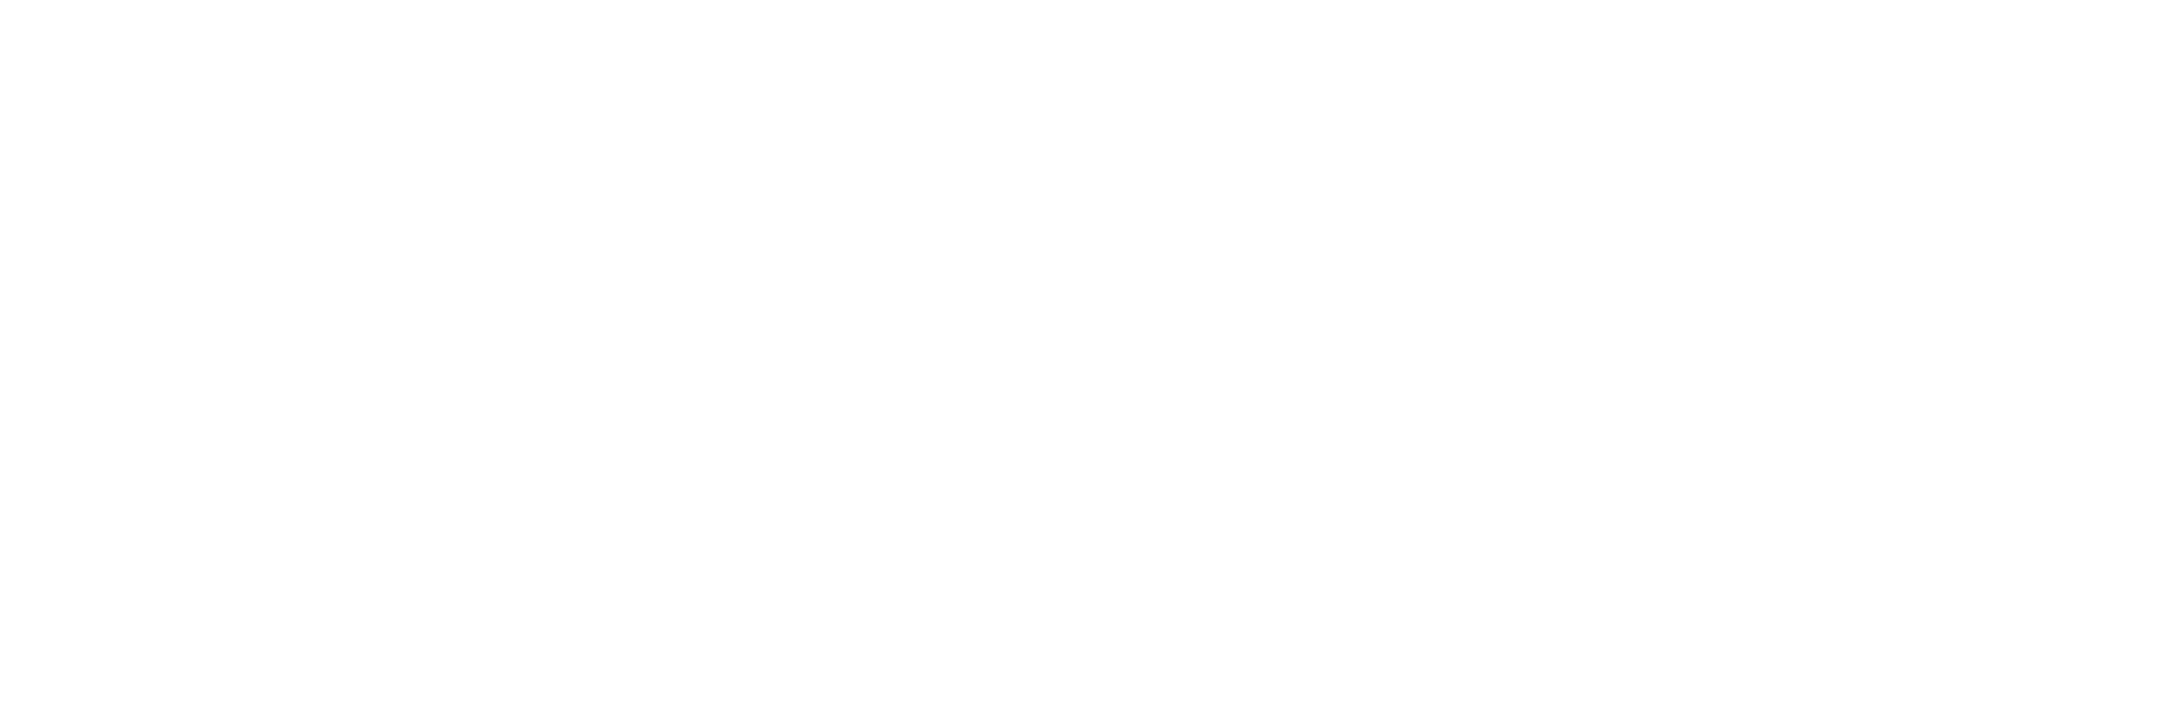
\includegraphics[width=1.04\paperwidth]{building-gate-white.png}};
  \end{tikzpicture}
  \vskip2.2cm
  \begin{center}
    {\Huge\bfseries\color{white}感谢聆听，敬请指正！}\\[1.8ex]
    {\large\color{white}Q \& A}\\[1.5ex]
    {\footnotesize\color{white!70}Hunan University of Arts and Science}
  \end{center}
\end{frame}

\end{document}
